\documentclass[a4paper]{article}

\usepackage[utf8]{inputenc}
\usepackage[T1]{fontenc}
\usepackage{textcomp}
\usepackage[italian]{babel}
\usepackage{amsmath, amssymb}
\usepackage{siunitx}
\usepackage{caption}
\usepackage{graphicx}
\usepackage{subcaption}
%dark mode
\usepackage{darkmode}


% figure support
\usepackage{import}
\usepackage{xifthen}
\pdfminorversion=7
\usepackage{pdfpages}
\usepackage{transparent}
\newcommand{\incfig}[1]{%
    \def\svgwidth{\columnwidth}
    \import{./figures/}{#1.pdf_tex}
}

\pdfsuppresswarningpagegroup=1

\begin{document}

\section{Introduzione}
Il primo insieme di esperienze volge a verificare, tramite l'utilizzo di circuiti a
corrente contuinua, fenomeni elettromagnetici. Più precisamente le misure effettuate sono mirate a:
\begin{itemize}
	\item valutare le caratteristiche degli strumenti di misura e verificare la legge di Ohm
	\item realizzare un partitore resistivo e studiarne il funzionamento
	\item misurare la caratteristica tensione-corrente di un diodo
	\item osservare gli effetti del campo magnetico generato da una spira percorsa da corrente

\end{itemize}

\section{Legge di Ohm}
\subsection{Obiettivo}
Misurare la relazione corrente-tensione ai capi di un resistore, utilizzando due diverse configurazioni del circuito per l'inserimento degli strumenti di misura
(voltometro e amperometro). A partire dai dati raccolti e dal loro confronto con quanto previsto dalla Legge di Ohm, valutare come la non idealità dei multimetri incida sulle misure.
%Considerare poi anche resistenze composite: in serie o in parallelo. (POSSIAMO EVITARE)
\subsection{Metodo}
Abbiamo innanzitutto costruito il circuito utilizzato per le misurazioni: abbiamo collegato l'alimentatore da banco, il quale fungeva da generatore di tensione, alla breadboard, tramite connettori a banana,
e la breadboard alla cassetta di resistenze mediante due cavi semplici, così da poter variare agevolmente la resistenza inserita nel circuito.
Per poter poi quantificare la relazione corrente-tensione abbiamo inserito nel circuito il voltometro, rappresentato dal multimetro palmare, e l'amperometro, rappresentata dal multimetro da banco.
Il collegamento con gli strumenti di misura è stato effettuato utilizzando due diverse configurazioni. Nella configurazione \ref{fig:1} il voltometro è stato collegato in parallelo con la resistenza;
nella configurazione \ref{fig:2} in parallelo con il generatore.
\begin{figure}[htbp]
	\centering
	\begin{subfigure}[b]{0.45\textwidth}
		\includegraphics[width=\textwidth]{conf_1.jpg}
		\caption{configurazione 1}
		\label{fig:1}
	\end{subfigure}
	\hfill
	\begin{subfigure}[b]{0.45\textwidth}
		\includegraphics[width=\textwidth]{conf_2.jpg}
		\caption{configurazione 2}
		\label{fig:2}
	\end{subfigure}
	\caption{configurazioni di misura ideali}
	\label{fig:prima}
\end{figure}
Per entrambe le configurazioni abbiamo raccolto almeno dieci misure della coppia corrente-tensione per due diversi resistori, uno con resistenza piccola (10 Ohm) e uno con resistenza grande (1MOhm).
Nell'utilizzare il carico resistivo più basso è stato possibile variare la tensione soltanto in un range ristretto di valori,
al fine di non raggiungere valori elevati di V così da evitare il passaggio di correnti troppo intense attraverso l'alimentatore o il multimetro da banco.
Abbiamo poi proceduto a determinare la resistenza interna dei multimetri, in modo tale da poterle confrontare con le resistenze inserite all'interno del circuito.
Sia amperometro che voltometro nel caso reale si comportano infatti come delle resistenze, identificate come \( \mathit{R_a} \) e \( \mathit{R_v} \),
seppur idealmente gli strumenti di misura non dovrebbero influire sulle misure di corrente e tensione.
Lo schema reale, in quale tiene conto della presenza dei multimetri all'interno del circuito, è mostrato in figura \ref{fig:3}.
\begin{figure}[htbp]
	\centering
	\begin{subfigure}[b]{0.45\textwidth}
		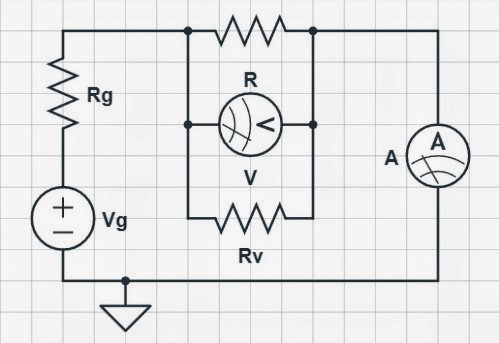
\includegraphics[width=\textwidth]{conf_1_bias.jpg}
		\caption{configurazione 1 con resistenze multimetri}
		\label{fig:a}
	\end{subfigure}
	\hfill
	\begin{subfigure}[b]{0.45\textwidth}
		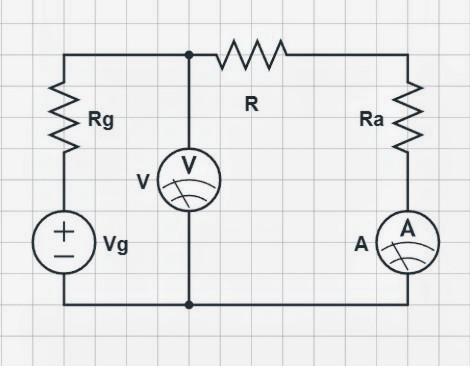
\includegraphics[width=\textwidth]{conf_2_bias.jpg}
		\caption{configurazione 2}
		\label{fig:b}
	\end{subfigure}
	\caption{configurazioni di misura reali}
	\label{fig:3}
\end{figure}
A partire dall'analisi circuitale della configurazione reale abbiamo quindi ricavato la relazione necessaria a determinare le resistenze interne \( \mathit{R_a} \) e \( \mathit{R_v} \).
Definita \( \mathit{I} \) la corrente che circola all'interno del circuito, \( \mathit{V} \) la differenza di potenziale applicata ai suoi capi, e \( \mathit{R} \) la resistenza propria del resistore
si ha:
\begin{align*}
	 & R_a = \frac {V}{I} - R & \quad \text{e} \quad R_v = \frac {I}{V} - frac{1}{R}
\end{align*}
Per determinare \( \mathit{R_v} \) è stata utilizzata la configurazione \ref{fig:a},
applicando la legge di Ohm alla tratto di circuito contenente le resistenze \( \mathit{R} \) e \( \mathit{R_v} \), tra loro in parallelo.
Al contrario, per ricavare \( \mathit{R_a} \), le misurazioni sono state effettuate utilizzando la configurazione \ref{fig:b},
sfruttando sempre la legge di Ohm, ma considerando la resistenza equivalente alla serie delle resistenze \( \mathit{R} \) e \( \mathit{R_a} \).
In entrambi i casi abbiamo raccolto le misure della coppia \( \mathit{I-V} \) per 5 valori distinti di \( \mathit{R} \), impostata dalla cassetta di resistenze.
\subsection{Dati}
\subsection{Analisi dati}
\subsection{Conclusione}


%%%%%%%%%%%%%%%%%%%%%%%%%%%%%%%%%%%%%%%%%%%%%%%%%%%%%%%%%%%%%%%%%%%%%%%%%%%%%%%%%%%%%%%%%%%%%%%%%%
\section{Partitore resistivo}
\subsection{Obiettivo}
Realizzare un circuito contenente tre diverse resistenze: \emph{R1, R2, Rload} strutturato come in figura \ref{fig:4}.
Il circuito deve essere dimensionato in modo tale che la caduta di potenziale ai capi della resistenza di carico \( \mathit{Vload} \) non dipenda dal valore di resistenza del carico.
Inoltre \( \mathit{R1} \) e \( \mathit{R2} \) devono essere scelte in modo che \( \mathit{Vin} \) sia circa \( \mathit{0.5 Vout} \).
\( \mathit{Vin} \) rappresenta la caduta di potenziale ai capi di \( \mathit{R1} \), mentre \( \mathit{Vout} \)indica la caduta di potenziale dovuta sia a \( \mathit{R1} \) che a \( \mathit{R2} \).
\begin{figure}[htbp]
	\centering
	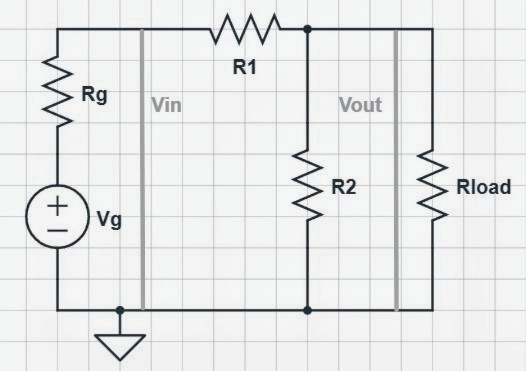
\includegraphics[width=0.5\textwidth]{partitore.png}
	\caption{Partitore resistivo}
	\label{fig:4}
\end{figure}
\subsection{Metodo}
Abbiamo realizzato il partitore resistivo utilizzando la breadbord, nella quale abbiamo inserito le resistenze \( \mathit{R1} \) e \( \mathit{R2} \),
e collegandola al generatore e alla cassetta di resistenze, scelta per rappresentare Rload così da poterne variare agevolmente i valori.
Al fine da rendere il valore della differenza di potenziale \( \mathit{Vload} \) costante, cioè indipendente da \( \mathit{Rload} \),
\( \mathit{Rload} \) deve assumere valori molto elevati, così che la corrente scorra prettamente nel tratto di circuito non contenente \( \mathit{Rload} \), e quindi non si abbia caduta di potenziale ai suoi capi.
Di fatto la corrente sceglie il percorso contenente \( \mathit{R1} \) e \( \mathit{R2} \).
Per avere \( \mathit{Vin ∼ 0.5Vout} \) le due cadute di tensione ai capi di \( \mathit{R1} \) e \( \mathit{R2} \) devono essere identiche, ossia, essendo attraversate dalla stessa corrente, \( \mathit{R1=R2} \).
Utilizzando le resistenze a disposizione abbiamo potuto garantire soltanto \( \mathit{R1∼R2} \), e non una esatta corrispondenza, infatti \( \mathit{R1=21.67 Ohm} \) e \( \mathit{R"=21.65 Ohm} \).
Dopo aver realizzato il partitore resistivo sulla breadboard, per verificare che esso rispetti le caratteristiche richieste, è stato necessario inserirvi il voltometro,
così da poter misurare i valori di \( \mathit{Vin} \) e \( \mathit{Vout} \). Per misurare \( \mathit{Vin} \) il voltometro è stato inserito in parallelo con l'alternatore,
mentre per la misura di \( \mathit{Vout} \) lo abbiamo collegato in parallelo con \( \mathit{Vload} \) (e quindi anche con la resistenza equivalente a \( \mathit{R1} \) e \( \mathit{R2} \)).
Abbiamo quindi effettuato 5 misure di \( \mathit{Vin} \) e \( \mathit{Vout} \) al variare di \( \mathit{Rload} \) tra 1 MOhm e 5 MOhm, e tenendo costante la tensione erogata dal generatore.
\subsection{Dati}
Nella tabella sottostante sono riportati i valori di \emph{Vin, Vout} e \emp {Rload} con i rispettivi errori.
Le incertezze di \( \mathit{Vin} \) e \( \mathit{Vout} \) sono state stimate utilizzando la sensibilità del voltometro, quindi \( \mathit{\delta_Vin=\delta_Vout=0.001 V} \);
mentre per determinare \( \mathit{\delta_Rload} \) abbiamo preso in considerazione l'errore relativo dell'1\% indicato sulla cassetta di resistenze.
%tabella con dati e errori (calcolare errore non relativo su R)
\subsection{Analisi dati}
\subsection{Conclusione}
Come si può osservare dai dati il valore della resistenza di carico non è completamente ininfluente su \( \mathit{Vload} \).
Al variare di \( \mathit{Rload} \) si hanno infatti fluttuazioni di \( \mathit{Vload} \); indice del fatto che, seppur \( \mathit{Rload} \) sia molto elevata, essa ha un valore finito e quindi
parte della corrente continua a fluire all'interno del componente resistivo. A conferma di ciò possiamo osservare come si raggiungano valori di \( \mathit{Vload} \) più alti all'aumentare di \( \mathit{Rload} \).
Inoltre come atteso per \( \mathit{R1∼R2} \) si ha \( \mathit{Vin ∼ 0.5Vout} \).

%%%%%%%%%%%%%%%%%%%%%%%%%%%%%%%%%%%%%%%%%%%%%%%%%%%%%%%%%%%%%%%%%%%%%%%%%%%%%%%%%%%%%%%%%%
\section{Caratteristica tensione-corrente di un diodo}
\subsection{Obiettivo}
Misurare tensione e corrente ai capi di un diodo e verificare che le informazioni raccolte rispettino quanto previsto dalla legge di Shockley: \(I = I_0 \left( e^{\frac{qV}{gkT}} - 1 \right)\).
Dove \( I \) è la corrente che attraversa il diodo mentre \( V \) è la tensione applicata. \( I_0 \) indica invece la corrente di saturazione inversa, \( g \) è una costante dipendente dal diodo,
\( k \) è la costante di Boltzmann (\( 1.38 \times 10^{-23} \, \text{J/K} \)), \( T \) è la temperatura in Kelvin, e \( q \) è la carica dell'elettrone (\( 1.60 \times 10^{-19} \)).
Utilizzare poi i dati per stimare la costante del diodo \( g \) e la corrente di saturazione inversa \( I_0 \).
\subsection{Metodo}
Abbiamo innanzitutto realizzato il circuito, ripetendo la proceduta utilizzata per la verifica della Legge di Ohm, inserendo all'interno della breadboard il diodo e scollegandola dalla cassetta di resistenze.
Per compiere le misurazioni di corrente e tensione sono state utilizzate per il collegamento dei multimetri sia la configurazione \ref{fig:1} che la configurazione \ref{fig:2},
per ciascuna delle quali abbiamo raccolto 21 misure della coppia \( I-V \). A partire dai valori di tensione e corrente abbiamo poi ricavato la resistenza equivalente,
dipendente dalla tensione tramite la relazione \( R_eq = \frac {V}{I} \), di conseguenza non costante; il diodo rappresenta infatti un componente non Ohmico.
Dal confronto di \(R_eq\) con le resistenze interne degli strumenti di misura è stato possibile valutare quale configurazione garantisse un bias minore sulle misure.
Per \(R_eq\) basse rispetto alla resistenza del voltometro si ottengono risultati più accurati scegliendo la configurazione \ref{fig:1}, in quanto la configurazione \ref{fig:2}
fornirebbe misure di \( V \) non corrispondenti alla differenza di potenziale ai capi del diodo, ma anzi alla serie tra \(R_eq\) e \(R_a\).
Al contrario per \(R_eq\) alte rispetto alla resistenza dell'amperometro, è preferibile la configurazione \ref{fig:2}.
Infatti se si utilizzasse la configurazione \ref{fig:1} l'amperometro misurerebbe una corrente che non corrisponde a quella che scorre attraverso il diodo,
poichè essa andrebbe a dividersi tra il tratto di circuito contenente \(R_v\) e quello contenente \(R_eq\).





%%%%%%%%%%%%%%%%%%%%%%%%%%%%%%%%%%%%%%%%%%%%%%%%%%%%%%%%%%%%%%%%%%%%%%%%%%%%%%%%%%%%%%%%%%


\section{Campo magnetico indotto da corrente}
\subsection{Obiettivo}
Verificare che il passaggio di corrente in una bobina generi un campo magnetico al suo interno.
Sfruttare una bussola per attuare le misurazioni, osservando come la corrente in circolo nella bobina incida sull'orientazione di un ago magnetico posto al suo interno.
\subsection{Metodo}
Abbiamo disposto il cellulare con l’app bussola sul supporto in modo tale che la bussola si trovasse al centro della bobina e che la direzione nord-sud da essa indicata
fosse perpendicolare all'asse del solenoide. In questo modo il campo magnetico generato dal passaggio di corrente (diretto lungo l'asse della bobina) aveva direzione perpendicolare
al campo magnetico terrestre (diretto lungo la direzione nord-sud). Abbiamo poi collegato la bobina all’alimentatore in regime di corrente continua e ne abbiamo aumentato gradualmente il valore,
osservando una progressiva rotazione dell'ago magnetico. Così facendo abbiamo raccolto 25 coppie di valori corrente-angolo di rotazione.
I valori di corrente sono stati utilizzati per determinare l'intensità del campo magnetico interno al solenoide, ricavato a partire dalla relazione \( B_s = \frac {\mu_0NI}{L} \),
dove \(\mu_0\) rappresenta la permeabilità magnetica del vuoto, \( \mathit{I} \) la corrente,
mentre \( \mathit{N=21} \) e \( \mathit{L=0.05m} \) indicano rispettivamente il numero di spire e la lunghezza del solenoide.
A partire dalle rotazioni è invece stata calcolata la tangente di ogni angolo.
\subsection{Dati}
Nella tabella e nel grafico sottostanti sono riportati i valori di corrente \( \mathit{I} \) e dell'angolo di rotazione \(\theta\).
Per la misura di entrambi abbiamo considerato come errore la sensibilità degli strumenti:
\( \mathit{\delta_I=0.01A} \)(sensibilità del generatore di corrente) e \( \mathit{\delta_\theta=0.02rad} \)(sensibilità della bussola).
%tabella (mettere angoli in radianti)
%grafico (mettere angoli in radianti)
\subsection{Analisi dati}
Abbiamo riportato in figura (x) i valori di \( \mathit{B_s} \) e \( \mathit{tan(\theta)} \) con i rispettivi errori.
Per ricavare l'incertezza su\( \mathit{tan(\theta)} \) e \( \mathit{B_s} \) sono state utilizzate le formule:
\[ \delta_tan = \frac {1}{1+\theta^2}\delta_\theta \]
\[ \delta_B_s = \frac {\mu_0N}{L}\delta_I \]
%tabella con valori di Bsolenoide e tangente +- loro errori
Tali dati sono stati poi interpolati con una legge di tipo lineare.
Ci aspettiamo infatti che essi siano legati dalla relazione \( tan(\theta) = \frac {B_s}{B_t} \) (dove \( \mathit{B_t} \) indica il campo magnetico terrestre),
la quale esprime come la presenza di un campo magnetico esterno perpendicolare al campo terrestre causi uno spostamento angolare.
%figura x (grafico con barre di errore) e retta
I risultati dell'interpolazione sono osservabili in seguito.
\( \mathit{m} \) indica il coefficiente angolare della retta e \( \mathit{a} \) la sua intercetta,
\( \mathit{\delta_m} \) e \( \mathit{\delta_q} \) i loro errori.
%tabella con valori parametri retta e loro errore
\subsection{Conclusione}
A partire dai parametri ricavati tramite l'interpolazione lineare abbiamo potuto determinare una stima del campo magnetico terrestre;
possiamo infatti dedurre il campo magnetico terrestre dal coefficiente angolare della retta che meglio approssima la relazione tra i dati.
Risulta \( \B_t = \frac {1}{m} \) con errore \( \delta_B_t = \frac {1}{m^2}\delta_m \).
I valori ottenuti sono raccolti nella tabella sottostante.
%tabella con campo terrestre e suo errore
%Dal momento che il campo magnetico terrestre assume un valore compreso tra \( \mathit{2.5*10^-5} \) e \( \mathit{6.5*10^-5 Tesla} \), 
%quanto ricavato sperimentalmente risulta confrontabile con il modello reale.











%resistenza attesa 1 mega ohm, con errore 1\%
%cofigurazione 2 (quella giusta con voltometro in parallelo al generatore)

\centering
\begin{tabular}{|c|c|c|c|c|}
	\hline
	$R_{\text{atteso}}$            & $R_1$                           & $P_1$ & $R_2$ & $P_2$ \\
	\hline
	$1000 \pm 10 \si{\kilo\ohm}$   & $908.5 \pm 0.95 \si{\kilo\ohm}$ & $1$   &
	$999.2 \pm 1.1 \si{\kilo\ohm}$ & $0.061$                                                 \\
	\hline
	$10 \pm 0.1 \si{\ohm}$         &                                 &       &       &       \\
	\hline
\end{tabular}
\captionof{table}{Verifica legge di Ohm}
\label{tab:Verfica legge di Ohm}






\subsection{}

\end{document}
